\documentclass{ctexart}
\usepackage[a4paper,total={6in,8in}]{geometry}
\usepackage{fancyhdr}
\usepackage[table,xcdraw]{xcolor}
\usepackage{diagbox}
\usepackage[utf8]{inputenc}
\usepackage{ctex}
\usepackage{color}
\usepackage{subfigure}
\usepackage{cite}
\usepackage{graphicx}
\usepackage{arydshln}
\usepackage{amsfonts}
\usepackage{fontspec}
\setmainfont{Times New Roman}
\newfontfamily\timesfont{Times New Roman}
\usepackage{CJK}
\usepackage{indentfirst}
\usepackage{amsmath}
\usepackage{mathrsfs}
\usepackage{multirow}
\usepackage{svg}
\usepackage{amsfonts}
\usepackage{geometry}
\usepackage{hyperref}
\usepackage{mathabx}
\usepackage{cases}
\definecolor{cherry}{HTML}{c93756}
\usepackage{minipage-marginpar}
\usepackage{xcolor}
% 导入包
\usepackage{hyperref}
% 格式设置
\hypersetup{hidelinks,
	colorlinks=true,
	allcolors=blue,
	pdfstartview=Fit,
	breaklinks=true}



\begin{document}

\begin{titlepage}
    \title{{\fontsize{28}{32}\selectfont\kaishu 机器人学 \\ \fontsize{20}{24}\selectfont\kaishu{作业5:运动学轨迹规划}}}
    \date{} % delete date as you want
    \maketitle
    \vspace{-7em}
    \begin{center}
      \fontsize{18}{22}\selectfont
      \textbf{\timesfont Robotics (2023-2024-2) \\
      Homework 5: Kinematic Trajectory Planning}
    \end{center}
    
    \begin{figure}[h]
        \centering
        
\includegraphics[width=0.45\textwidth]{Image/校标-校徽.png}
    \end{figure}
    \begin{center}
      \hspace{6em}
      \renewcommand{\arraystretch}{2}
      \begin{tabular}{rl}
      \fontsize{16}{50}\selectfont\heiti 姓名:& \fontsize{16}{24}\selectfont\heiti 赵四维 \\
      \fontsize{16}{24}\selectfont\heiti 学号:& \fontsize{16}{24}\selectfont 521021910696 \\
      \fontsize{16}{24}\selectfont\heiti 班级:& \fontsize{16}{24}\selectfont ME3403-01 \\
      \fontsize{16}{24}\selectfont\timesfont E-mail:& \fontsize{16}{24}\selectfont racheus.11@sjtu.edu.cn \\
      \end{tabular}
    \end{center}
    \begin{center}
      \fontsize{16}{24}\selectfont\timesfont \today
    \end{center}
\end{titlepage}

\pagenumbering{arabic}

\newpage
% \tableofcontents


\newpage
\pagestyle{fancy}
\fancyhf{}
\fancyhead[L]{ME3403-01}
\fancyhead[C]{机器人学Homework7}
\fancyhead[R]{赵四维 521021910696}
\fancyfoot[C]{\thepage}
\section*{Question 1}
已知旋转矩阵
\begin{equation*}
	R = \begin{bmatrix}
		0 & 0 & 1 \\
		0 & -1 & 0 \\
		1 & 0 & 0
	\end{bmatrix}
\end{equation*}

且$R = e^{\hat{\omega}\theta},\omega \in \mathbb{R}^3 , \theta \in [0,2\pi )$,求所有满足条件的$\omega$和$\theta$。

\textbf{Solution:}
首先,由旋转矩阵$R$,我们可以验算其满足正交性
\begin{equation*}
	r_i \cdot r_j = \begin{cases}
		1 & ,i = j \\
		0 & ,i \neq j
	\end{cases}
\end{equation*}

因此\textcolor{cherry}{$R \in SO(3)$}(\textbf{IMPORTANT!})

接下来,求取矩阵的特征值

\begin{equation}
	|\lambda \boldsymbol{I} -\boldsymbol{R}| = \left| \begin{matrix}
		\lambda & 0 & -1 \\
		0 & \lambda+1 & 0 \\
		-1 & 0 & \lambda
	\end{matrix} \right| = (\lambda+1)(\lambda^2 - 1) = 0
\end{equation}

因此矩阵的特征值为$\lambda_1 = \lambda_2 = -1,\lambda_3 = 1$,由此,矩阵的迹(trace)为
\begin{equation}
	\text{tr}(R) = \sum_{n = 1}^{3} \lambda_n = -1-1+1 = -1
\end{equation}

由于有 $\text{tr}(R) = -1$, 我们可以得到$cos \theta =-1$,由$\theta$的取值范围$[0,2\pi)$,我们可以得到$\theta = \pi$。

由于特征值排列方式的不同,对角化矩阵的方式也有所不同,我们可以得到几个不同的结果:
\begin{enumerate}
	\item $\omega = \frac{1}{\sqrt{2(1+R_{33})}}\begin{bmatrix}
		      R_{13} \\
		      R_{23} \\
		      1+R_{33}
	      \end{bmatrix} =\frac{\sqrt{2}}{2} \begin{bmatrix}
		      1 \\
			  0 \\
			  1
	      \end{bmatrix}$,带入验证此时的R是满足条件的。
	\item $\omega = \frac{1}{\sqrt{2(1+R_{22})}}\begin{bmatrix}
		      R_{12} \\
		      R_{22} \\
		      1+R_{32}
	      \end{bmatrix}$ ,代入$R_{22} = -1$,此时分母为0,因此此时的$\omega$不满足条件。
	\item $\omega = \frac{1}{\sqrt{2(1+R_{11})}}\begin{bmatrix}
		      R_{11} \\
		      R_{21} \\
		      1+R_{31}
	\end{bmatrix} = \frac{\sqrt{2}}{2} \begin{bmatrix}
		0 \\
		0 \\
		2
	\end{bmatrix}$,带入验证,此时$\omega$既不是单位向量,也无法得到$R$。
		
\end{enumerate}
综上,有且仅有1满足条件,再由于$-\omega$也满足条件,因此有两个解$\omega = \pm \frac{\sqrt{2}}{2} \begin{bmatrix}
	1 \\
	0 \\
	1
\end{bmatrix},\theta = \pi$.

\section*{Question 2}
已知$v_1,v_2 \in \mathbb{R}^3$,且满足
\begin{equation*}
	v_2 = e ^ {\hat{\omega} \theta} v_1
\end{equation*}

其中$\omega = [\frac{2}{3},\frac{2}{3},\frac{1}{3}]^T,v_1=[1,0,1]^T,v_2=[0 ,1 ,1]^T$,求$\theta$。

\textbf{Solution:}
首先,我们可以求取$R$的表达式

\begin{equation*}
	\begin{aligned}
		R &= e^{[\hat{\omega}] \theta} = I + [\hat{\omega}]sin\theta + [\hat{\omega}]^2(1-cos\theta)\\
		&= I + sin \theta \begin{bmatrix}
			0 & -\omega_3 & \omega_2 \\
			\omega_3 & 0 & -\omega_1 \\
			-\omega_2 & \omega_1 & 0
		\end{bmatrix} + (1-cos\theta)  \begin{bmatrix}
			0 & -\omega_3 & \omega_2 \\
			\omega_3 & 0 & -\omega_1 \\
			-\omega_2 & \omega_1 & 0
		\end{bmatrix}^2\\
		&= \begin{bmatrix}
			1 & 0 & 0 \\
			0 & 1 & 0 \\
			0 & 0 & 1
		\end{bmatrix} + sin\theta \begin{bmatrix}
			0 & -\frac{1}{3} & \frac{2}{3} \\
			\frac{1}{3} & 0 & -\frac{2}{3} \\
			-\frac{2}{3} & \frac{2}{3} & 0
		\end{bmatrix} + (1-cos\theta) \begin{bmatrix}
			-\frac{5}{9} &  \frac{4}{9} &  \frac{2}{9} \\
			\frac{4}{9} &  -\frac{5}{9} &  \frac{2}{9} \\
			\frac{2}{9} &  \frac{2}{9} &  -\frac{8}{9}
		\end{bmatrix}\\
		&= \begin{bmatrix}
			1+\frac{5}{9}(cos\theta -1) & \frac{1}{3}sin\theta + \frac{4}{9}(1-cos\theta) & \frac{2}{3}sin\theta + \frac{2}{9}(1-cos\theta) \\
			\frac{1}{3}sin\theta + \frac{4}{9}(1-cos\theta) & 1+\frac{5}{9}(cos\theta -1) & -\frac{2}{3}sin\theta + \frac{2}{9}(1-cos\theta) \\
			-\frac{2}{3}sin\theta + \frac{2}{9}(1-cos\theta) & \frac{2}{3}sin\theta + \frac{2}{9}(1-cos\theta) & 1+\frac{8}{9}(cos\theta -1)
		\end{bmatrix}
	\end{aligned}
\end{equation*}

再代入题目中的关系式$v_2 = Rv_1$,我们可以得到
\begin{equation*}
	\begin{cases}
		1+\frac{5}{9}(cos\theta -1)+\frac{2}{3} sin\theta + \frac{2}{9}(1-cos\theta) = 0\\
		\frac{1}{3}sin\theta + \frac{4}{9}(1-cos\theta) - \frac{2}{3}sin\theta + \frac{2}{9}(1-cos\theta) = 1\\
		-\frac{2}{3}sin\theta + \frac{2}{9}(1-cos\theta) + 1 + \frac{8}{9}(cos\theta -1) = 1
	\end{cases}
\end{equation*}

由上述方程组,我们可以得到$sin \theta = -1,cos \theta = 0$,因此$\theta = \frac{3}{2}\pi$。(假设角度条件同第一题,$\theta \in [0,2\pi)$)
	
\section*{Question 3}
下图为二自由度机械臂,$l_0,l_1,l_2$分别为连杆的长度,$\theta_1,\theta_2$分别为连杆的角度。

\begin{figure}[h]
	\centering
	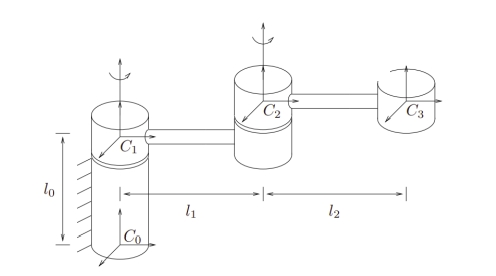
\includegraphics[width=0.6\textwidth]{Image/1.png}
	\caption{二自由度机械臂}
\end{figure}

\begin{enumerate}
	\item 求取$C_3$相对于$C_0$的位置和姿态。
	\item 求取$C_3$相对于$C_0$的spatial velocity。
	\item 求取$C_3$相对于$C_0$的body velocity。
\end{enumerate}

\textbf{Solution:}
1. 由题目中的图示和指数坐标方法,
\begin{equation*}
	g_{st}(0) = \left[\begin{array}{ccc:c}
		1 & 0 & 0 & 0\\
		0 & 1 & 0 & l_1+l_2\\
		0 & 0 & 1 & l_0\\
		\hdashline 
		0 & 0 & 0 & 1\\ 
		\end{array}\right],\omega_1 = \omega_2 = \begin{bmatrix}
			0 \\
			0 \\
			1
		\end{bmatrix}
\end{equation*}

由Revolute Joint有$\xi_i= \begin{bmatrix}
	\omega_i \times q_i \\
	\omega_i
\end{bmatrix}$,$e^{\xi_i \theta_i}=\begin{bmatrix}
	e^{\hat{\omega_i}\theta_i} & (I - e^{\hat{\omega_i}\theta_i})(\omega_i \times q_i) + \omega_i \omega_i^T q_i \theta_i \\
	0 & 1
\end{bmatrix}
$,我们可以得到
\begin{equation*}
	\xi_1 = \begin{bmatrix}
		0 \\
		0 \\
		0 \\
		0 \\
		0 \\
		1
	\end{bmatrix},\xi_2 = \begin{bmatrix}
		l_1\\
		0 \\
		0 \\
		0 \\
		0 \\
		1
	\end{bmatrix},
	e^{\xi_1 \theta_1} = \begin{bmatrix}
		c_1 & -s_1 & 0 & 0 \\
		s_1 & c_1 & 0 & 0 \\
		0 & 0 & 1 & 0 \\
		0 & 0 & 0 & 1
	\end{bmatrix},e^{\xi_2 \theta_2} = \begin{bmatrix}
		c_2 & -s_2 & 0 & l_1s_2 \\
		s_2 & c_2 & 0 & l_1(1-c_2) \\
		0 & 0 & 1 & 0 \\
		0 & 0 & 0 & 1
	\end{bmatrix}
\end{equation*}

thus,$g_{st}(\theta_1,\theta_2)=e^{\xi_1 \theta_1}e^{\xi_2 \theta_2}g_{st}(0)$,其中
\begin{equation*}
	e^{\xi_1 \theta_1}e^{\xi_2 \theta_2} = \begin{bmatrix}
		c_1c_2-s_1s_2 & -c_1s_2-s_1c_2 & 0 & l_1s_2c_1+l_1s_1(c_2-1) \\
		s_1c_2+c_1s_2 & -s_1s_2+c_1c_2 & 0 & l_1s_2s_1+l_1c_1(1-c_2) \\
		0 & 0 & 1 & l_0 \\
		0 & 0 & 0 & 1
	\end{bmatrix}
	=\begin{bmatrix}
		c_{12} & s_{12} & 0 & l_1(s_{12}-s_1)\\
		s_{12} & -c_{12} & 0 & l_1(c_1-c_{12})\\
		0 & 0 & 1 & 0 \\
		0 & 0 & 0 & 1
	\end{bmatrix}
\end{equation*}

由分块矩阵的乘法,记$e^{\xi_1 \theta_1}e^{\xi_2 \theta_2} = \begin{bmatrix}
	R & \boldsymbol{p_1} \\
	0 & 1
\end{bmatrix},g_{st}(0)=\begin{bmatrix}
	I & \boldsymbol{p_2} \\
	0 & 1
\end{bmatrix}$,我们可以得到$C_3$相对于$C_0$的位置和姿态

\begin{equation*}
	\begin{aligned}
		g_{st}(\theta_1,\theta_2) &= \begin{bmatrix}
			R & \boldsymbol{p_1}  \\
			0 & 1
		\end{bmatrix} \begin{bmatrix}
			I & \boldsymbol{p_2} \\
			0 & 1
		\end{bmatrix}
		= \begin{bmatrix}
			R & \boldsymbol{p_1} +R\boldsymbol{p_2}  \\
			0 & 1
		\end{bmatrix}\\
		&= \begin{bmatrix}
			c_{12} & -s_{12} & 0 & -l_2s_{12}-l_1s_1 \\
			s_{12} & c_{12} & 0 & l_2c_{12}+l_1c_1\\
			0 & 0 & 1 & l_0 \\
			0 & 0 & 0 & 1
		\end{bmatrix}
	\end{aligned}
\end{equation*}

2. 由现代机器人学spatial velocity的定义,

\begin{equation*}
	\begin{aligned}
		\hat{V}^S_{ab}= \dot{g}_{ab}g_{ab}^{-1} = \begin{bmatrix}
			\dot{R}R^T & -\dot{R}R^T\boldsymbol{p_{ab}}+\dot{\boldsymbol{p_{ab}}} \\
			0 & 0
		\end{bmatrix}
	\end{aligned}
\end{equation*}

其中$\dot{R} = \begin{bmatrix}
	-(\omega_1 + \omega_2)s_{12} & -(\omega_1 + \omega_2)c_{12} & 0 \\
	(\omega_1 + \omega_2)c_{12} & -(\omega_1 + \omega_2)s_{12} & 0 \\
	0 & 0 & 0
\end{bmatrix}$,$\dot{\boldsymbol{p_{ab}}} = \begin{bmatrix}
	-l_2(\omega_1 + \omega_2)c_{12} - l_1\omega_1c_1 \\
	-l_2(\omega_1 + \omega_2)s_{12} - l_1\omega_1s_1 \\
	0
\end{bmatrix}$.

注意上式中的$\omega_1 = \dot{\theta_1},\omega_2 = \dot{\theta_2}$,因此我们可以得到
\begin{equation*}
	\dot{R}R^T= \begin{bmatrix}
		-(\omega_1 + \omega_2)s_{12} & -(\omega_1 + \omega_2)c_{12} & 0 \\
		(\omega_1 + \omega_2)c_{12} & -(\omega_1 + \omega_2)s_{12} & 0 \\
		0 & 0 & 0
	\end{bmatrix}\begin{bmatrix}
		c_{12} & -s_{12} & 0 \\
		s_{12} & c_{12} & 0 \\
		0 & 0 & 1
	\end{bmatrix}^T= \begin{bmatrix}
		0 & -(\omega_1+\omega_2) & 0 \\
		(\omega_1+\omega_2)& 0 & 0 \\
		0 & 0 & 0
	\end{bmatrix}
\end{equation*}

\begin{equation*}
	\dot{\boldsymbol{p_{ab}}} - \dot{R}R^T\boldsymbol{p_{ab}} = \begin{bmatrix}
		-l_2(\omega_1 + \omega_2)c_{12} - l_1\omega_1c_1 \\
		-l_2(\omega_1 + \omega_2)s_{12} - l_1\omega_1s_1 \\
		0
	\end{bmatrix}-\begin{bmatrix}
		-l_2(\omega_1 + \omega_2)c_{12} - l_1\omega_1c_1 \\
		-l_2(\omega_1 + \omega_2)s_{12} - l_1\omega_1s_1 \\
		0
	\end{bmatrix} = \begin{bmatrix}
		l_1\omega_2c_1 \\
		l_1\omega_2s_1 \\
		0
	\end{bmatrix}
\end{equation*}

因此,我们可以得到$C_3$相对于$C_0$的spatial velocity

\begin{equation*}
	\begin{aligned}
		\hat{V}^S_{30} &= \begin{bmatrix}
			0 & -(\omega_1+\omega_2) & 0 & l_1\omega_2c_1 \\
			(\omega_1+\omega_2)& 0 & 0 & l_1\omega_2s_1 \\
			0 & 0 & 0 & 0 \\
			0 & 0 & 0 & 0
		\end{bmatrix}
	\end{aligned}
\end{equation*}

如果写成向量形式:
\begin{equation*}
	\begin{aligned}
		V^S_{30} &=\begin{bmatrix}
			v_{30}^S \\
			\omega_{30}^S
		\end{bmatrix} =
		\begin{bmatrix}
			l_1\omega_2s_1 \\
			l_1\omega_2c_1 \\
			0 \\
			0\\
			0 \\
			\omega_1+\omega_2 
		\end{bmatrix}
	\end{aligned}
\end{equation*}

3. 由现代机器人学body velocity的定义,
\begin{equation*}
	\begin{aligned}
		\hat{V}^b_{ab}=g_{ab}^{-1} \dot{g}_{ab} = \begin{bmatrix}
			R^T\dot{R} & -R^T\boldsymbol{p_{ab}} \\
			0 & 0
		\end{bmatrix}
	\end{aligned}
\end{equation*}

只用算

\begin{equation*}
	\begin{aligned}
	R^T\dot{R} &=\begin{bmatrix}
		c_{12} & -s_{12} & 0 \\
		s_{12} & c_{12} & 0 \\
		0 & 0 & 1
	\end{bmatrix}^T
	\begin{bmatrix}
		-(\omega_1 + \omega_2)s_{12} & -(\omega_1 + \omega_2)c_{12} & 0 \\
		(\omega_1 + \omega_2)c_{12} & -(\omega_1 + \omega_2)s_{12} & 0 \\
		0 & 0 & 0
	\end{bmatrix}\\&= \begin{bmatrix}
		0 & -(\omega_1+\omega_2) & 0 \\
		(\omega_1+\omega_2)& 0 & 0 \\
		0 & 0 & 0
	\end{bmatrix}\\
	R^T \dot{\boldsymbol{p_{ab}}} &= \begin{bmatrix}
		c_{12} & -s_{12} & 0 \\
		s_{12} & c_{12} & 0 \\
		0 & 0 & 1
	\end{bmatrix}^T
	\begin{bmatrix}
		-l_2(\omega_1 + \omega_2)c_{12} - l_1\omega_1c_1 \\
		-l_2(\omega_1 + \omega_2)s_{12} - l_1\omega_1s_1 \\
		0
	\end{bmatrix}\\ &= \begin{bmatrix}
		-l_2(\omega_1 + \omega_2)-l_1\omega_1cos(\theta_1+\theta_2-\theta_1) \\
		l_1\omega_1sin(\theta_1+\theta_2-\theta_1) \\
		0
	\end{bmatrix}
	= \begin{bmatrix}
		-l_2(\omega_1 + \omega_2)-l_1\omega_1cos\theta_2 \\
		l_1\omega_1sin\theta_2 \\
		0
	\end{bmatrix}
\end{aligned}
\end{equation*}

所以我们可以得到$C_3$相对于$C_0$的body velocity
\begin{equation*}
	\begin{aligned}
		\hat{V}^b_{30} &= \begin{bmatrix}
			0 & -(\omega_1+\omega_2) & 0 & -l_2(\omega_1 + \omega_2)-l_1\omega_1cos\theta_2 \\
			(\omega_1+\omega_2)& 0 & 0 & l_1\omega_1sin\theta_2 \\
			0 & 0 & 0 & 0 \\
			0 & 0 & 0 & 0
		\end{bmatrix}
	\end{aligned}
\end{equation*}

如果写成向量形式:
\begin{equation*}
	\begin{aligned}
		V^b_{30} &=\begin{bmatrix}
			v_{30}^b \\
			\omega_{30}^b
		\end{bmatrix} =
		\begin{bmatrix}
			-l_2(\omega_1 + \omega_2)-l_1\omega_1cos\theta_2 \\
			l_1\omega_1sin\theta_2 \\
			0 \\
			0\\
			0 \\
			\omega_1+\omega_2 
		\end{bmatrix}
	\end{aligned}
\end{equation*}
\end{document}

